% Horizon penetrating coordinates (vs. Schwarzschild coordinates)
% for a black hole spacetime, with excision
% Author: Jonah Miller
\documentclass[tikz,border=0pt]{standalone}
\usepackage{tikz}
\usepackage{pgf}
\usetikzlibrary{arrows}
\usetikzlibrary{arrows.meta}
\usetikzlibrary{automata}
\usetikzlibrary{positioning}
\usetikzlibrary{decorations.markings}
\usepackage{pgfplots}
\usepackage{xcolor}

%\tikzset{>={Latex[length=3mm]}}

\begin{document}
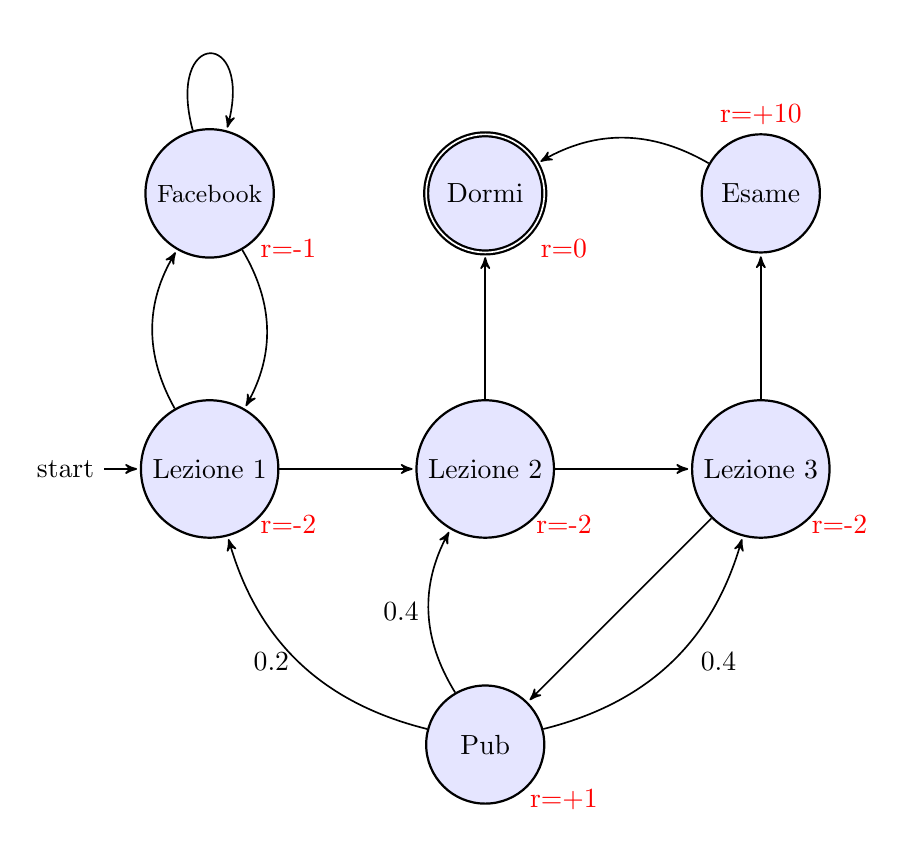
\begin{tikzpicture}[->, >=stealth', shorten >= 1pt, node distance=3.5cm, semithick]
\tikzstyle{every state} = [draw=black, text=black, minimum size=1.5cm, thick, fill=blue!10]

\node[state] (A) {\small Facebook\normalsize};
\node[state,initial] (B)[below of=A] {Lezione 1};
\node[state] (C)[right of=B] {Lezione 2};
\node[state] (D)[right of=C] {Lezione 3};
\node[state] (E)[above of=D] {Esame};
\node[state] (F)[below of=C] {Pub};
\node[state, accepting] (G)[above of=C] {Dormi};

\draw (A) node[text=red, xshift=1cm, yshift=-0.7cm)] {r=-1};
\draw (B) node[text=red, xshift=1cm, yshift=-0.7cm)] {r=-2};
\draw (C) node[text=red, xshift=1cm, yshift=-0.7cm)] {r=-2};
\draw (D) node[text=red, xshift=1cm, yshift=-0.7cm)] {r=-2};
\draw (E) node[text=red, xshift=0cm, yshift=1cm)] {r=+10};
\draw (F) node[text=red, xshift=1cm, yshift=-0.7cm)] {r=+1};
\draw (G) node[text=red, xshift=1cm, yshift=-0.7cm)] {r=0};


\path (A) edge[bend left] node[right]{} (B)
			edge[loop above] node[xshift=15pt,yshift=-12pt]{}	(A)
	(B) edge[bend left] node[left]{} (A)
		edge[] node[above]{} (C)
	(C) edge[] node[left]{} (G)
		edge[] node[above]{} (D)	
	(D) edge[] node[below,right]{} (F)
		edge[] node[right]{} (E)
	(E) edge[bend right] node[above]{} (G)
	(F) edge[bend left] node[left]{0.2} (B)
		edge[bend left] node[left]{0.4} (C)
		edge[bend right] node[right=7pt]{0.4} (D) 
	;

\end{tikzpicture}
\end{document}